\NeedsTeXFormat{LaTeX2e}
\documentclass{fac}
\ifprodtf \else \usepackage{latexsym}\fi
\usepackage[utf8]{inputenc}
\usepackage{graphicx}
\usepackage{bm}
\usepackage{amssymb,amsmath}
\usepackage{topcapt,booktabs}
\usepackage{tikz}
\usepackage{pgfplots} 
\usepackage{listings}
\usepackage{appendix}
\pgfplotsset{compat=newest}
\usetikzlibrary{shapes,arrows,positioning}
\usetikzlibrary{shapes.arrows,patterns}

\newcommand{\abs}[1]{\lvert#1\rvert}
\newcommand{\floor}{\mathop{\textrm{floor}}\nolimits}

\title[Transcendental Verification using Theorem Proving]{Formal Verification of Transcendental Fixed and Floating Point Algorithms using an Automatic Theorem Prover}


\author[Samuel Coward]
    {Samuel Coward$^1$, Lawrence Paulson$^2$, Theo Drane$^3$ and Emiliano Morini$^3$\\
     $^1$Faculty of Mathematics, University of Cambridge,\\
     $^2$Computer Laboratory, University of Cambridge,\\
     $^3$Cadence Design Systems, Cambridge\\}

\correspond{Samuel Coward, 58 Grove Hall Court, 2 Hall Road, St Johns Wood, London, NW8 9NY, UK.\\
            e-mail: s.coward111@gmail.com}

\pubyear{2020}
\pagerange{\pageref{firstpage}--\pageref{lastpage}}

\begin{document}
\label{firstpage}

\makecorrespond

\maketitle

\begin{abstract}
We present a method for formal verification of transcendental hardware and software algorithms that scales to higher precision without suffering an exponential growth in runtimes. A class of implementations using piecewise polynomial approximation to compute the result is verified using MetiTarski, an automated theorem prover, which verifies a range of inputs for each call. The method was applied to commercial implementations from Cadence Design Systems with significant runtime gains over exhaustive testing methods and was successful in proving that the expected accuracy of one implementation was overly optimistic.
\end{abstract}
\begin{keywords}Theorem prover; Transcendental functions; Floating point algorithms; Hardware implementation
\end{keywords}

%%%%%%%%%%%%%%%%%%%%%%%%%%%%%%%%%%%%%%%%%%%%%%%%%%%%%%%%%%%%%%%%%%%%%%%%%%%%%%%%%%%%%%%%%%%%%%%%%%%%%%%%%%%%%%%%%%%%%%%%%%%%%%%%%%%%%%%%%%%%%%%%
%INTRODUCTION
%%%%%%%%%%%%%%%%%%%%%%%%%%%%%%%%%%%%%%%%%%%%%%%%%%%%%%%%%%%%%%%%%%%%%%%%%%%%%%%%%%%%%%%%%%%%%%%%%%%%%%%%%%%%%%%%%%%%%%%%%%%%%%%%%%%%%%%%%%%%%%%%
\section{Introduction}
\label{intro}
Formal verification of floating point operations is becoming ever more challenging as hardware designs reach levels of complexity only previously seen in software. Its importance in industry is well known, exemplified by the Pentium floating point division bug \cite{pratt1995anatomy}. The bulk of this research was conducted during a project at Cadence Design Systems. Building upon this, we present a new approach to the verification of fixed and floating point transcendental algorithms. This technique should be viable for verifying high precision algorithms, as our findings suggest that runtimes will not rise exponentially with the precision.  Our experiments cover implementations of logarithms and the sine function; however, the methodology can also be applied to many different functions implemented using algorithms of the form described in \S \ref{trans functs}. Verification of logarithm implementations is a relevant problem as it finds applications in fields such as digital signal processing and 3D graphics \cite{lewis1995114,harris2001powering}. In addition, it can be very simple to implement, with one of the simplest examples of a floating point logarithm just using the exponent as the integer part of the result combined with a lookup table for the most significant bits (msb) of the significand, to generate the fractional part \cite{harris2001powering}.
\begin{equation*}
    \log(2^{\textit{exp}} \times 1.sig) \approx \textit{exp} + LUT(\textit{sig}[msb])
\end{equation*}

% Traditional verification techniques
Traditional techniques rely on exhaustive testing of all inputs to verify such algorithms, but this can be resource intensive, perhaps prohibitively so. The Multiple Precision Floating-Point Reliable (MPFR) library is a C library for multiple-precision floating point computations with correct rounding \cite{fousse2007mpfr}, and is widely used as a reference for many verification tasks. For example, some of the industrial implementations presented here were verified by comparing the outputs to the MPFR library. We shall see that the methodology used in this paper performs more efficiently in particular cases. 

% Functions to verify
The paper will focus on implementations of transcendental functions in hardware that rely on piecewise polynomial approximations. Many elementary functions are traditionally calculated in software \cite{10.5555/1096483,gal1991accurate}, but for numerically intensive algorithms such implementations may simply be too slow, leading to the development of dedicated hardware \cite{tang1991table,strollo2011elementary,pineiro2004algorithm}. Although primarily focusing on hardware, some software implementations may be amenable to the verification approach presented here, as we shall see in \S\ref{gappa}. De Dinechin, Lauter and Melquiond verified a CRlibm double precision library function using the Gappa proof assistant \cite{daramy2009cr,5483294}. Their approach is potentially the most similar method (in execution) to ours and therefore we will also use our method to verify the same function. All the examples considered here use a binary representation, but the simplest decimal floating point implementations, that convert to binary, use the binary algorithm, then convert back to decimal would also be amenable \cite{5223332}. Other decimal floating point implementations appear to rely more on the digit-recurrence algorithm \cite{5223326,5710893}, which is more challenging to reduce to a series of inequalities since decisions are typically made at each iteration based on information from the previous iterations.

% Commented out as not sure it is the right place
%In floating point arithmetic, the upper most portion of the input significand is passed to a lookup table which outputs a number of coefficients. The remainder of the input is then used to compute a polynomial approximation to %the exact result. Scaling to handle the exponent is often computed in a separate section of the code. Such an approach is easy to verify using the methodology described in this paper, but will hold for any implementation %where it is possible to abstract an underlying mathematical model that can be expressed as a system of inequalities for verification purposes.

% MetiTarski Introduction
To produce the required proofs we use MetiTarski~\cite{akbarpour2010metitarski}, an automatic theorem prover for real valued analytic functions, such as cosine and logarithm. It's a combination of a resolution theorem prover and a decision procedure for the theory of real closed fields (RCF). A field is real closed if every positive number has a square root, which is equivalent to saying that it has the same first-order properties as the reals. The resolution prover at the base of MetiTarski is Joe Hurd's Metis \cite{metis_theorem_prover}, which is modified in several respects \cite{akbarpour2008metitarski}. One key modification is to the ordering of the resolution prover \cite{ludwig2007extension}, which encourages the replacement of supported functions by bounds. The inbuilt axioms are primarily upper and lower bounds on a set of supported functions. The choice of these bounds was carefully considered. Many are based on the bounds proposed by Daumas, Lester and Munoz \cite{daumas2008verified}; these are typically derived from Taylor series. Other bounds are obtained from continued fraction expansions, for example
\[\frac{1}{2} \leq x \leq 1 \implies \frac{x-1}{x} \leq \ln(x) \leq \frac{3x^2-4x+1}{2x^2}.\]

The resolution prover applies the axioms replacing any supported funtions and generates polynomial inequalites. With the problem reduced to the theory of RCFs, the decision procedure is then sufficient to finalise the proof. Conjectures are passed to MetiTarski as a set of inequalities which are transformed by replacing any special function by an appropriate bound. Typically proofs are found in a few seconds \cite{akbarpour2009applications}, but if MetiTarski is unable to prove a conjecture it does not mean that the conjecture is false. For verification it is important that MetiTarski produces machine readable proofs that include algebraic simplification, decision procedure calls, and resolution rules \cite{denman2009formal}. MetiTarski is among a limited number of automated tools supporting transcendental functions. Examples include the first-order logic automated reasoning tool \texttt{dReal} \cite{gao2013dreal} and an approach to Satisfiability Modulo the theory of transcendental functions, which used properties from the MetiTarski suite as benchmarks \cite{cimatti2017satisfiability}. Our initial research inspired a new enhancement to MetiTarski, with the addition of axioms to bound the floor function. The main benefit of the update, for this paper, is to simplify the syntax and construction of our conjectures, with this contribution being the first application of the new axioms.

% Summary of paper sections
In the following section we will discuss the common approaches to implementations of elementary functions. In \S \ref{Method}, we will describe the verification methodology of this paper with actual applications and results of using this method presented in \S \ref{Apps}. Lastly we will compare our approach to other theorem proving verification methods in \S \ref{gappa} and \S \ref{Related}.

%%%%%%%%%%%%%%%%%%%%%%%%%%%%%%%%%%%%%%%%%%%%%%%%%%%%%%%%%%%%%%%%%%%%%%%%%%%%%%%%%%%%%%%%%%%%%%%%%%%%%%%%%%%%%%%%%%%%%%%%%%%%%%%%%%%%%%%%%%%%%%%%
% Transcendental Function Implementations
%%%%%%%%%%%%%%%%%%%%%%%%%%%%%%%%%%%%%%%%%%%%%%%%%%%%%%%%%%%%%%%%%%%%%%%%%%%%%%%%%%%%%%%%%%%%%%%%%%%%%%%%%%%%%%%%%%%%%%%%%%%%%%%%%%%%%%%%%%%%%%%%

\section{Transcendental Function Implementations}
\label{trans functs}

% General methods
As mentioned above, transcendental functions are commonly implemented in software, however the numerical algorithms used in software are often unsuitable for hardware. One example, using Chebyshev series expansion, would result in a high area circuit due to its use of a variety of expensive operations such as floating point multiplication \cite{fowkes1993hardware}. There are lots of different hardware algorithms to implement these functions, but a large proportion fall into one of the following categories: digit-recurrence \cite{bajard1994bkm,1030708}, CORDIC  (Coordinate Rotation DIgital Computer) \cite{volder1959cordic,andraka1998survey,10.1145/1478786.1478840} or table-lookup \cite{tang1991table,story1999new}. A comparison of the different algorithms is beyond the scope of this paper but has been tackled by other authors \cite{tang1991table,pineiro2004algorithm}. We will focus on table-lookup algorithms, as they are broadly used and are the most amenable to our methodology .

%Table lookup outline
Tang's 1991 paper provided a general framework for implementing a function $f$ on an interval $I$, which most table driven algorithms use to some degree \cite{tang1991table}. According to Tang, typical table-lookup algorithms have a set of \textit{breakpoints} $c_k \in I$ for $k=1, 2, ... N$, along with a table of approximations $T_k$, such that $f(c_k) \approx T_k$. Given $x \in I$, the algorithm uses the following steps to calculate $f(x)$:
%Evaluation of steps to calculate a table-lookup algorithm.
\begin{enumerate}

\item \textbf{Reduction}: Solve $k = min_k \abs{x-c_k}$, then apply a \textit{reduction transformation} $r = R(x,c_k)$.

\item \textbf{Approximation}: Calculate $f(r)$ using an approximating function $p(r)$, often a polynomial is used here.

\item \textbf{Reconstruction}: Using a reconstruction function $S$, which is determined by $f$ and $R$, a final approximation is found.
\begin{align*}
    f(x) &= S(f(c_k),f(r)) \\
         &\approx S(T_k,p(r)).
\end{align*}

\end{enumerate} 

%Sizes of lookup tables and industrial apps
In the rest of the paper, Tang describes algorithms for $2^x, \log(x),$ and $\sin{(x)}$, for relatively narrow intervals. In these examples, tables ranging in size from 32 to 64 entries are used. To support wider intervals, further transformations of the arguments to these narrow domains are necessary. For example, a common sine transformation is to subtract an integer multiple, $N$, of $\frac{\pi}{2}$ from the argument, $x$, such that $x-N \times \frac{\pi}{2} \in [-\frac{\pi}{4}, \frac{\pi}{4}]$ \cite{harrison2006floating,harrison2000formal}. Having reduced the argument to this narrow domain, the question remains about how to best approximate the function in this interval. Polynomials are a common choice, and to calculate the coefficients there are a number of approaches. Some use Remez algorithm to generate the coefficients of the minmax polynomial \cite{veidinger1960numerical,tang1991table}, while others opt to use carefully rounded coefficients from the function's Chebyshev expansion \cite{378099}. For the IA-64 architecture, Intel provided a library of table based algorithms for computing several transcendental functions \cite{harrison1999computation}. The tables used in this library range in size from 24 to 256 double extended entries, for the exponential and logarithm, respectively.

% LUT with piecewise-poly approx
Table based algorithms have been further developed and modified to use lookup tables to construct piecewise polynomial approximations to some elementary functions \cite{strollo2011elementary,pineiro2005high}. The reduction step still uses the breakpoint method, but the table no longer returns just an approximation, $T_k$, it now returns multiple polynomial coefficients for each lookup. Strollo, De Caro and Petra present, alongside their algorithm, many different divisions of the input domain. For example, to compute $\ln(1+x)$ for $x\in[0,1]$ using a piecewise-quadratic approximation, accurate to 24 fractional bits, they required 128 table entries of coefficients \cite{strollo2011elementary}. In the industrial implementation described below, a table containing 32 breakpoints is used. 

In this paper, the input to the function will often be represented in floating point format \cite{goldberg1991every}, which stores a number as $(-1)^{s} \times 2^{e-b} \times 1.\textit{significand}$. In IEEE-754 standard single precision, $s$ is a single bit representing the sign, the exponent $e$ is an 8 bit integer, the bias $b$ is a constant equal to 127, and the significand is 23 bits long. The implementations of the logarithm verified in this paper rely on the following identity.
\begin{align*}
    \log(2^{\textit{exp}} \times 1.\textit{significand}) &= \log(2^{\textit{exp}}) + \log(1.\textit{significand}) \\
                                                &= \textit{exp} + \log(1.\textit{significand}),
\end{align*}
The reconstruction step then simply involves adding the integer exponent to an approximation to $\log(1.\textit{significand})$. This approximation passes the top $k$ bits of the significand to a lookup table, which returns coefficients for a degree $m$ polynomial, evaluated using the remaining low bits of the significand. Clearly, if the polynomial approximation contains a zeroth order term, then that coefficient is equivalent to the $T_k$ described above. As this approach is essentially an enhancement to the method described by Tang, the verification of these piecewise polynomial LUT methods could also be adapted to the simpler LUT methods.


%%%%%%%%%%%%%%%%%%%%%%%%%%%%%%%%%%%%%%%%%%%%%%%%%%%%%%%%%%%%%%%%%%%%%%%%%%%%%%%%%%%%%%%%%%%%%%%%%%%%%%%%%%%%%%%%%%%%%%%%%%%%%%%%%%%%%%%%%%%%%%%%
% Verification Methodology
%%%%%%%%%%%%%%%%%%%%%%%%%%%%%%%%%%%%%%%%%%%%%%%%%%%%%%%%%%%%%%%%%%%%%%%%%%%%%%%%%%%%%%%%%%%%%%%%%%%%%%%%%%%%%%%%%%%%%%%%%%%%%%%%%%%%%%%%%%%%%%%%
\section{Verification Methodology}
\label{Method}
% Translation into MetiTarski problem
Given an implementation of a transcendental function following the outline above, we obtain an abstraction that is verifiable using MetiTarski. If the top $k$ bits of the significand are passed to a lookup table, for a fixed 8-bit exponent and sign bit, we reduce the verification problem to $2^k$ calls to MetiTarski. Therefore, the  full verification over all inputs is reduced to 
just $2^{k+8+1}$ MetiTarski conjectures to be proven. In some cases, verification over all such inputs is not necessary: a bespoke hand proof may be able to confirm the correctness of the results for exponent scalings. Of course, most verification tasks use massively parallel processing to reduce the runtimes. Similar methods may be used to reduce the runtimes in our approach, as the conjectures passed to MetiTarski are independent of each other. In nearly all commercial implementations, $k$ is relatively small as lookup tables can have high ROM demands \cite{strollo2011elementary}. Assuming that our interpolation coefficients are stored in a file, and we can express the problem as a set of inequalities, the procedure follows the same basic outline. \\

% Method outline
\noindent\textbf{Procedure Outline} (see Figure \ref{procedure_flow})
\begin{enumerate}
\item Write a template problem for the inequalities to be proven, with placeholders for all the relevant interpolation coefficients and upper bit values.
\item Use a wrapper script to read the coefficients and replace them in the template problem to generate the full set of MetiTarski problems.
\item Run the Perl script that accompanies MetiTarski to test all of the problems.
\item Refine error modeling on problems that are not proven and return to step 1.
\item Exhaustively test regions where MetiTarski was unsuccessful.
\end{enumerate}  

% Flow diagram for procedure
\begin{figure} \label{procedure_flow}
\centering
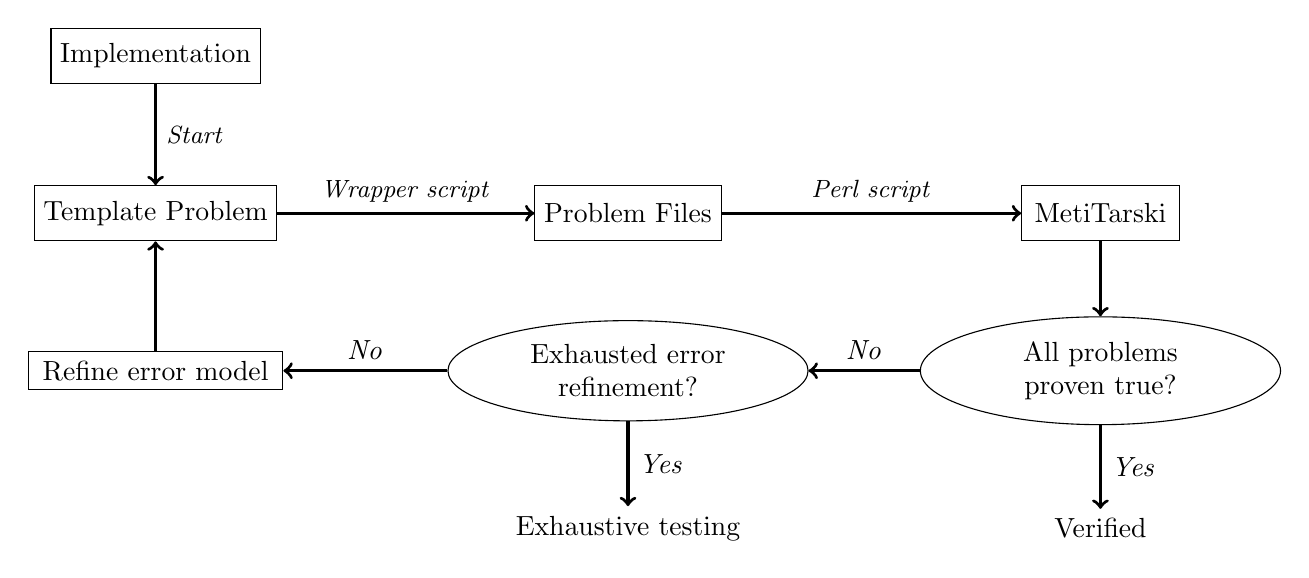
\begin{tikzpicture}

% Top row
\node [shape=rectangle,draw = black, minimum width = 1cm,minimum height=0.7cm] at (-1,8.5) (impl) {Implementation};

% Second row
\node [shape=rectangle,draw = black, minimum width = 1cm,minimum height=0.7cm] at (-1,6.5) (temp) {Template Problem};
\node [shape=rectangle,draw = black, minimum width = 1cm,minimum height=0.7cm] at (5,6.5) (prob) {Problem Files};
\node [shape=rectangle,draw = black, minimum width = 2cm,minimum height=0.7cm] at (11,6.5)   (metit) {MetiTarski};

% Third row
\node [shape=rectangle,draw=black,text width=3cm,text centered] at (-1,4.5) (refine)   {Refine error model};
\node [shape=ellipse,draw=black,text width=3cm,text centered] at (5,4.5)   (more_ref) {Exhausted error refinement?};
\node [shape=ellipse,draw=black,text width=3cm,text centered] at (11,4.5) (prove)    {All problems proven true?};

% Fourth row
\node [] at (5,2.5)   (test) {Exhaustive testing};
\node [] at (11,2.5) (verif) {Verified};

%Lines between input and LUT or final output box
\draw [->,very thick] (impl) -- (temp) node[midway,right] {\small \textit{Start}};
\draw [->,very thick] (temp) -- (prob) node[midway,above] {\small \textit{Wrapper script}};
\draw [->,very thick] (prob) -- (metit) node[midway,above] {\small \textit{Perl script}};
\draw [->,very thick] (metit) -- (prove) ;
\draw [->,very thick] (prove) -- (more_ref) node[midway,above] {\textit{No}};
\draw [->,very thick] (more_ref) -- (refine) node[midway,above] {\textit{No}};
\draw [->,very thick] (prove) -- (verif) node[midway,right] {\textit{Yes}};
\draw [->,very thick] (more_ref) -- (test) node[midway,right] {\textit{Yes}};
\draw [->,very thick] (refine) -- (temp);

\end{tikzpicture}

\caption{Flow diagram of the verification procedure. Always start by generating an initial template problem from the given implementation. \label{procedure}}
\end{figure}

% Introduction of toy implementation
To demonstrate the methodology, we analyse a toy implementation for computing the natural logarithm based on the outline above. The implementation takes as an input an 8 bit integer $x_0x_1...x_7$ and outputs an approximation to $\ln(1.x_0...x_7)$. The top four bits, $i = x_0..x_3$, are passed to a lookup table that returns the 10 bit interpolation coefficients $a_i, b_i, c_i$, for $i=0,...,15$. The coefficients are generated using a simple quadratic interpolation scheme. Writing $x=0.x_0...x_7$, the approximation generated is,
\[ \overline{\ln(1+x)}=c_i + b_i x +a_i x^2. \]
This example is designed to be simple to show the underlying principles of the verification methodology. Later, we shall adapt it to be more relevant to industrial implementations. In this case, the implementation is accurate to $2^{-10}$, which can easily be verified using exhaustive testing as the input space only contains $2^8$ values.

% Statement of problem to prove
\[\abs{\ln(1+x)-\overline{\ln(1+x)}} <2^{-10} \qquad (x= 0.x_0...x_7) \]

% Method description
The first step is to generate the template problem. In this problem, the upper bits are represented by a constant, $\_\_y=0.x_0...x_3$, and the lower bits, $X$, are modelled as a MetiTarski variable, to which we assign a specified range. The coefficients, which will be replaced in step 2 of the procedure, are just placeholders, $\_\_a, \_\_b$ and $\_\_c$. If this were a real hardware implementation the design could be improved by absorbing $\_\_y$, a constant, into the pre-calculated coefficients, resulting in a polynomial just in $X$.
% Template Problem
\[ 0\le X \le 2^{-4}-2^{-8} \implies \abs{\ln(1+\_\_y+X)-(\_\_c+\_\_b(\_\_y+X)+\_\_a(\_\_y+X)^2)} < 2^{-10} \]

% Wrapper script and MetiTarski Proofs
A wrapper script now generates the 16 MetiTarski problems, replacing the placeholders $\_\_a, \_\_b$ and $\_\_c$ with the actual coefficients from the LUT and $\_\_y$ with the relevant constant input to the LUT. A Perl script, which is supplied with MetiTarski, automates the calls to our prover, providing a true or false result for each problem. For our toy implementation, MetiTarski is able to provide proofs for all of these problems and therefore steps 4 and 5 of the procedure are rendered redundant. Next we enhance the toy implementation and start to see where the refinement step is useful. The total runtime was 5.3 seconds and no more than 0.4 seconds is spent on any one proof. On such a small input space, exhaustive search is quicker by several orders of magnitude, taking less than a tenth of a second. However, as we shall see, our technique does not suffer from exponentially increasing runtimes as we increase the precision of the implementation. 

% Enhanced Toy Implementation
With this basic understanding of the methodology, we shall make the toy implementation more realistic. Commercial hardware engineers have constraints on area and performance targets to meet, so they apply techniques to reduce the resource requirements. One of these is to truncate bits throughout the algorithm, reducing the number of adders required. This generally improves the performance but typically with some cost to the accuracy of the approximation. In our implementation, we choose appropriate terms to truncate in order to more closely replicate commercial algorithms. The new implementation returns an approximation of the form, 
% Approximation
\begin{equation} \label{update_toy}
\overline{\ln(1+x)}=c + 2^{-8} \lfloor{b(x_0...x_7)} \rfloor +a(0.x_0...x_5)^2. 
\end{equation}
In this case, the approximation is accurate to $2^{-7}$.

% Statement of accuracy
\[ \abs{\ln(1+x)-\overline{\ln(1+x)}} <2^{-7} \qquad (x= 0.x_0...x_7) \]

% Floor function 
This can easily be checked using exhaustive testing, but notice that the implementation uses bit truncation on the first and second order terms. Since MetiTarski has no understanding of the integers, such non-analytic functions are are difficult to model. In HOL Light, Harrison developed an entire theory of floating point arithmetic to more closely model the hardware he intended to verify \cite{harrison1999machine}. For our purposes, it was sufficient to explore only simple approximations and bounds to such arithmetic. Inspired by this research, MetiTarski now includes support for a floor function. MetiTarski understands functions via axioms that give upper and lower bounds, and in the case of the floor function we simply have $x-1< \floor(x)\le x$. It should be noted that this bound is poor when the inputs under investigation are close to 1, for example MetiTarski will fail to prove $\floor(0.5)\geq 0$.
However, for the examples investigated in this paper, such a bound is sufficient to verify the function to the same precision that can be verified via exhaustive testing. Therefore, using this function, it is possible to produce a MetiTarski conjecture. We now allow $X$ to be the integer value of the bottom 4 bits ($x_4x_5x_6x_7$) and $\_\_y$ the integer value of the top 4 bits ($x_0x_1x_2x_3 0000$), which, as before, determines the coefficients $\_\_a, \_\_b, \_\_c$. We now use the integer values of $X$ and $\_\_y$, because doing so allows us to model bit truncation using the floor function. Our new template problem is then, 
% Enhance toy template problem
\[
0\le X \le 15 \implies \abs{\ln(1+2^{-4}\_\_y+2^{-8}X) - M_1\_\ln(1+x)} <2^{-7} \qquad (x= 0.x_0...x_7)
\]
where,
\[
M_1\_\ln(1+x)=\_\_c+2^{-8}\floor(\_\_b(X+2^{4}\_\_y))+2^{-12}\_\_a(\floor(2^{-2}X+2^{2}\_\_y))^2.
\]

% Error correlation and flaw in its approach.
Using the floor function provides a simple, but usually effective model. However, this approach has an issue, which it shares with interval arithmetic, in that all correlation of errors is lost by this approach. To demonstrate this problem consider the following equation and MetiTarski floor function model of it, where $z$ is a 4 bit integer.
\[
(z>>1) - (z>>2) \rightarrow  \floor(\frac{1}{2}z) - \floor(\frac{1}{4}z)
\]
\[
\floor(\frac{1}{2}z) \in [\frac{1}{2}z-1, \frac{1}{2}z], \quad \floor(\frac{1}{4}z) \in [\frac{1}{4}z-1,\frac{1}{4}z]
\]

The floor function model indicates that this equation is bounded below by $\frac{1}{2}z - 1 - \frac{1}{4}z = \frac{1}{4}z - 1$. In actual fact the equation is bounded below by $\frac{1}{4}z - \frac{1}{4}$. This discrepancy is a result of disregarding any correlation between the two terms in the model. This issue also occurs in interval arithmetic, but fortunately we can deploy additional variables in our model which account for some of this correlation. Using two additional error variables our MetiTarski problem can model this behaviour more accurately.
\begin{align*}
(z>>1) - (z>>2) &\rightarrow \frac{1}{2}z - \epsilon_0 - (\frac{1}{4}z - \epsilon_1 - \frac{1}{2}\epsilon_0) \qquad z \in [0,15], \quad \epsilon_0 \in [0,\frac{1}{2}], \quad \epsilon_1 \in [0,\frac{1}{2}] \\   
                &=           \frac{1}{4}z + \epsilon_1 - \frac{1}{2}\epsilon_0 \in [\frac{1}{4}z - \frac{1}{4}, \frac{1}{4}z + \frac{1}{2}]
\end{align*}

%Error Variables
Essentially, the error variables, $\epsilon_0$ and $\epsilon_1$, bound bits 0 and 1 of the variable $z$, allowing us to attain the bound we found analytically above, tighter than the bound we found using the floor function approach. Clearly, if we were to introduce an error variable for every bit truncated, then the number of variables in our MetiTarski problem would grow to be huge for any real world design. This is problematic as MetiTarski runtimes can be doubly exponential in the number of variables, an inherent limitation of the decision procedure on which it relies. In addition, this approach to error modelling requires significantly more user input and skill than the simple floor function method. Intellectual effort is needed to calculate the correlation between error terms introduced in the hardware algorithm.

%Refinement Step
This example is intended to highlight the limitations of the floor function method, and to demonstrate that with additional human and computational effort it is possible to refine our error models. Returning to the procedure outline given above, the floor function method should be used to generate the initial template problem in step 1. If in step 3, MetiTarski fails to prove all the problems it is given, we can introduce error variables in our template problem to refine our error model. This is typically an iterative approach, as there is a tradeoff between the human effort required and the tightness of the error bounds. So there may be several rounds of error model refinement with MetiTarski runs until either, the problems are all proven or the error model refinements are exhausted. If, after exhausting all error model refinements, some of the MetiTarksi problems remain unproven, then the last step is to use exhaustive testing on the remaining regions. All this effort is typically not wasted, as proving a subset of the MetiTarski problems will reduce, possibly significantly, the size of the input space left for verification using exhaustive testing. In \S \ref{Apps}, we discuss a complex industrial implementation where this final exhaustive step was necessary to complete the verification.

To illustrate this approach, we model our updated implementation, eqn \ref{update_toy}, using error variables rather than the floor function. This yields a new MetiTarski problem,
\[
	0\le X \le 15 \hspace{0.1cm} \land \hspace{0.1cm} 0\le \epsilon_0<1\hspace{0.1cm} \land \hspace{0.1cm} 0\le \epsilon_1<1
	\implies \abs{\ln(1+2^{-4}\_\_y+2^{-8}X) - M_2\_\ln(1+x,\epsilon_0,\epsilon_1)} < 2^{-7}
\]
where, 
\[
M_2\_\ln(1+x,\epsilon_0,\epsilon_1)=\_\_c+2^{-8}(\_\_b(X+2^{4}\_\_y)-\epsilon_0)+2^{-12}\_\_a((2^{-2}X+2^{2}\_\_y)-\epsilon_1)^2.
\]

Surprisingly, for this particular problem, using additional error variables rather than the floor function actually had minimal impact on the overall runtime for the 16 problems. However, the floor function is a recent addition to MetiTarski and we may be able to improve its performance by fine-tuning its heuristic parameters. On industrial implementations, to limit the number of variables it was sometimes necessary to combine error variables and manually calculate an upper bound on these. This was often challenging: some of the error variables can be highly correlated. The floor function method makes the process of generating an initial template problem significantly simpler. For the industrial implementations verified in this paper, error variables were necessary, since tight error bounds were required.
\begin{figure}
\centering
\scalebox{0.9}{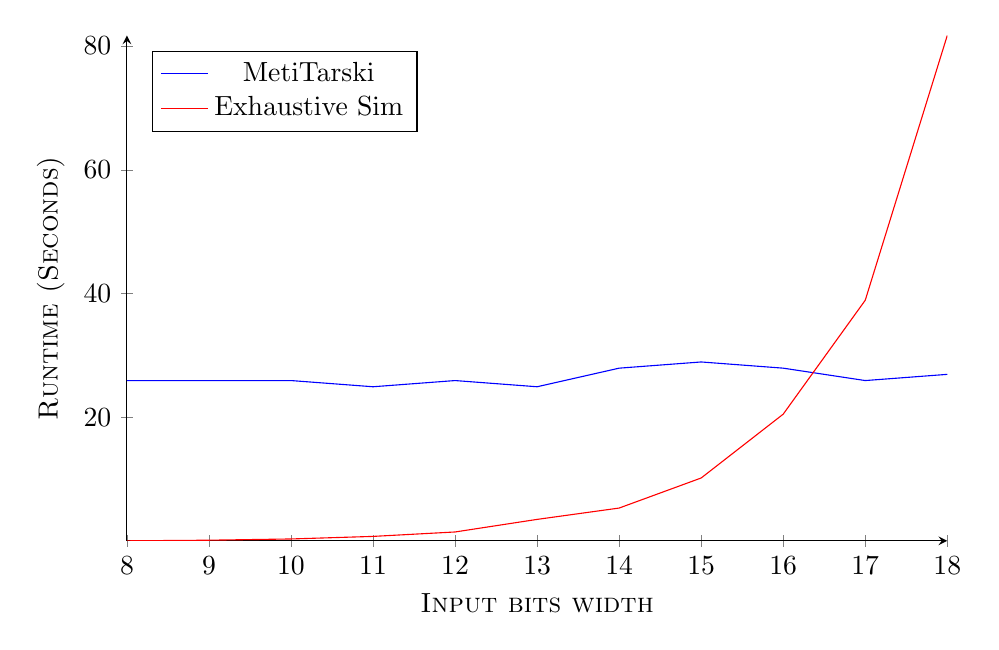
\begin{tikzpicture}
\begin{axis}[
    axis lines = left,
    xlabel = \textsc{Input bits width},
    ylabel = \textsc{Runtime (Seconds)},
    legend pos=north west,height=80mm, width=120mm]

\addplot[
    color=blue,
    ]
    coordinates {(8 ,26)(9 ,26)(10,26)(11,25)(12,26)(13,25)(14,28)(15,29)(16,28)(17,26)(18,27)   };
    \addlegendentry{MetiTarski}
\addplot[color=red,
        ]
        coordinates{(8 ,0.14548254013061523 )
(9 ,0.24578046798706055 )(10,0.4463155269622803  )
(11,0.8605005741119385  )(12,1.574721336364746   )
(13,3.603602409362793   )(14,5.432856559753418)
(15,10.283031702041626)(16,20.580944299697876)
(17,38.95604610443115)(18,81.67475938796997)

 };
        \addlegendentry{Exhaustive Sim}
\end{axis}
\end{tikzpicture}
}
\caption{A graph demonstrating the runtime comparison of the competing verification procedures on implementations of growing precision, results obtained running on a single core Intel I7-3517U \label{runtime_graph}}
\end{figure}

% Larger input space
To see why this technique is powerful, we extend the implementation above to larger input spaces. The approximation is essentially the same, using the same coefficients and lookup table, but our input now may be 10 bits rather than 8 bits, for example. Figure \ref{runtime_graph} compares the runtimes of our methodology and exhaustive testing as the input space grows. Notably, the MetiTarski method has roughly constant runtimes, as we expect: MetiTarski is an analytic tool, so increasing the space of discrete inputs only minimally alters the MetiTarski problems. Conversely, exhaustive testing runtimes suffer from exponential growth in the number of bits of the input. Of course, if the size of the lookup table increases, this will affect the MetiTarski runtimes as the number of problems will grow exponentially. The tables used in these algorithms are typically not prohibitively large, those referenced in \S 2 contained less than 256 entries, since large tables translate into additional silicon in hardware designs.


%%%%%%%%%%%%%%%%%%%%%%%%%%%%%%%%%%%%%%%%%%%%%%%%%%%%%%%%%%%%%%%%%%%%%%%%%%%%%%%%%%%%%%%%%%%%%%%%%%%%%%%%%%%%%%%%%%%%%%%%%%%%%%%%%%%%%%%%%%%%%%%%
% Applications and Discussion
%%%%%%%%%%%%%%%%%%%%%%%%%%%%%%%%%%%%%%%%%%%%%%%%%%%%%%%%%%%%%%%%%%%%%%%%%%%%%%%%%%%%%%%%%%%%%%%%%%%%%%%%%%%%%%%%%%%%%%%%%%%%%%%%%%%%%%%%%%%%%%%%
\section{Applications and Discussion}
\label{Apps}
% Introduction to section
We present some results from applying this methodology to the verification of several larger commercial implementations. The runtime results can be found in Table \ref{result} and demonstrate that the technique has real world relevance.

% Block diagram of implementation
\begin{figure}
\centering
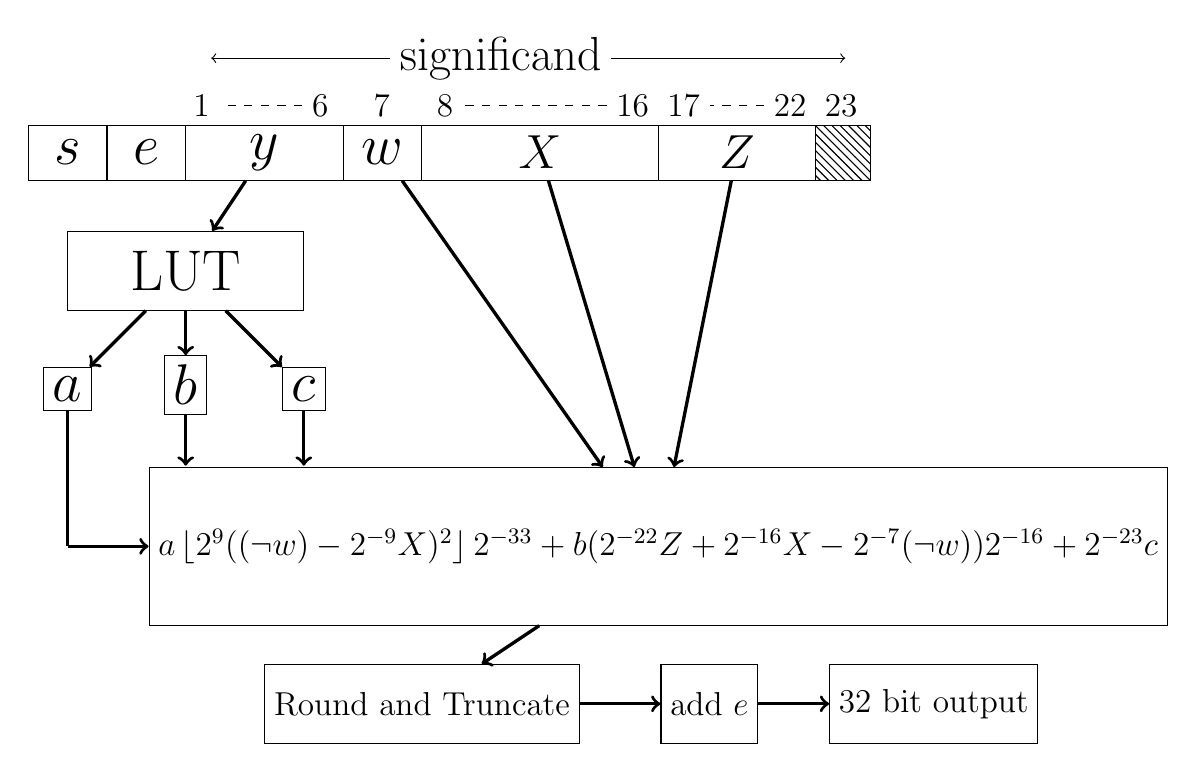
\begin{tikzpicture}
%draw input nodes
\node [shape=rectangle,draw = black, minimum width = 1cm,minimum height=0.7cm] at (0.5,6.5) {\huge $s$};
\node [shape=rectangle,draw = black, minimum width = 1cm,minimum height=0.7cm] at (1.5,6.5) {\huge $e$};
\node [shape=rectangle,draw = black, minimum width = 2cm,minimum height=0.7cm] at (3,6.5) (y) {\huge $y$};
\node [shape=rectangle,draw = black, minimum width = 1cm,minimum height=0.7cm] at (4.5,6.5) (w) {\huge $w$};
\node [shape=rectangle,draw = black, minimum width = 3cm,minimum height=0.7cm] at (6.5,6.5) (x) {\LARGE $X$};
\node [shape=rectangle,draw = black, minimum width = 2cm,minimum height=0.7cm] at (9,6.5) (z) {\LARGE $Z$};

\draw[pattern=north west lines, pattern color=black] (10,6.15) rectangle ++(0.7,0.7);


%\node at (0.5,7.5){sign};
%\node at (1.5,7.5){exp};
%\node at (8.5,8.1) {\huge mantissa};

%labels above inputs

\node at (6,7.7) (mant) {\LARGE significand};
\node at (2.2,7.7) (left_mant) {};
\node at (10.5,7.7) (right_mant) {};
\node at (10,7.1) (lowest) {\large 22 \hspace{0.1cm}23};
\node at (8,7.1) (low) {\large 16 \hspace{0.1cm}17};
\node at (4.5,7.1) (mid){\large 6 \hspace{0.3cm} 7 \hspace{0.32cm} 8};
\node at (2.2,7.1) (high) {\large 1};

\draw [dashed] (lowest) edge (low);
\draw [dashed] (low) edge (mid);
\draw [dashed] (mid) edge (high);
\draw [->] (mant) edge (left_mant);
\draw [->] (mant) edge (right_mant);

%draw lookup table with nodes output from LUT
\node [shape=rectangle,draw = black, minimum width = 3cm,minimum height=1cm] at (2,5) (lut) {\huge LUT};
\node [shape=rectangle,draw=black] at (0.5,3.5) (a) {\huge $a$};
\node [shape=rectangle,draw=black] at (2,3.55) (b) {\huge $b$};
\node [shape=rectangle,draw=black] at (3.5,3.5) (c) {\huge $c$};

%draw output box
\node [shape=rectangle,draw = black,minimum height=2cm] at (8,1.5) (poly) {\large $a\left \lfloor2^9((\neg{w})-2^{-9}X)^2\right \rfloor 2^{-33}+b(2^{-22}Z+2^{-16}X-2^{-7}(\neg{w}))2^{-16}+2^{-23}c$};

\node [shape=rectangle,draw = black,minimum height=1cm] at (5,-0.5) (round) {\large Round and Truncate};

\node [shape=rectangle,draw = black,minimum height=1cm] at (8.65,-0.5) (exp_scale) {\large add $e$};

\node [shape=rectangle,draw = black,minimum height=1cm] at (11.5,-0.5) (output) {\large 32 bit output};

%Lines between input and LUT or final output box
\draw [->,very thick] (y) edge (lut);
\draw [->,very thick] (x) edge (poly);
\draw [->,very thick] (w) edge (poly);
\draw [->,very thick] (z) edge (poly);
\draw [->,very thick] (poly) edge (round);
\draw [->,very thick] (round) edge (exp_scale);
\draw [->,very thick] (exp_scale) edge (output);


%Edges between LUT and outcomes
\draw [->,very thick] (lut) edge (a);
\draw [->,very thick] (lut) edge (b);
\draw [->,very thick] (lut) edge (c);
%Draw right angle edges
\draw [-,very thick] (a) edge (0.5,1.5);
\node at (2,2.4) (emptyb) {};
\draw [->,very thick] (b) edge (emptyb);
%\draw [-,very thick] (c) edge (3.5,1.5);
\node at (3.5,2.4) (emptyc) {};
\draw [->,very thick] (c) edge (emptyc);
\node at (0.38,1.5) (empty) {};
\draw [->,very thick] (empty) edge (poly);

\end{tikzpicture}

\caption{A description of the implementation of the floating point $\log_2$ which MetiTarski was used to verify. The input is a 32 bit floating point number where $s$ is the sign bit, $e$ is the exponent, $y$ is the top 6 bits of the significand and $w$, $X$ and $Z$ are divisions of the significand. The last bit is discarded.\label{block_diagram}}
\end{figure}

% Description of implementation
Figure \ref{block_diagram} gives a description of the floating point implementation verified using this methodology. This implementation was a release candidate for Cadence Design Systems. We see that the 23 bit significand is split into 4 used sections, whilst the last bit is discarded. The top 6 bits, $y$, are passed to the LUT which outputs 3 polynomial coefficients. Using these coefficients the algorithm computes a polynomial approximation to the logarithm. The split significand is used to reduce the number of operations along with a truncation of bits which are insignificant for the accuracy target. The accuracy target for the implementation was 4 ULPs (unit in last place) \cite{muller2010handbook}, which is why, for the following conjectures the bounds on the distance from the true logarithm are $2^{-21}(=4\times 2^{-23})$, since we consider inputs in the region [1,2). The exponent, $e$, in our input region is equal to the IEEE-754 bias $b$, yielding a zero exponent in the decoded value. This was the first implementation verified using the MetiTarski method, and as a result, when this was investigated the floor function was not supported. However, rather than calling the floor function explicitly the bounds on the calculations were calculated by hand and combined to yield a simple bound on the error in either direction. This is a labour intensive method, and was the inspiration behind the introduction of the floor function. This manual approach, resulted in two separate template problems. 

% Outline template problems
\begin{align*}
    \textrm{Template 1} &\Rightarrow approx \leq exact + 2^{-21} \\
    \textrm{Template 2} &\Rightarrow approx \geq exact - 2^{-21}
\end{align*}
\begin{multline*}
(\textrm{ }l=0.69314718055994530941723212145817\textrm{ } \&\textrm{ } 0\leq X \leq2^9-1\textrm{ } \& \textrm{ }0\leq Z \leq 2^6-1\textrm{ }) \Rightarrow \\ 
\textbf{Template 1} \\
  \textrm{ }  2^{-33} a\Big(2^9(1-w)+2X(w-1)+ 2^{-9}X^{2}\Big)   +  2^{-38} b\Big(Z +2^{6}X + 2^{15}(w-1)\Big)+  2^{-23}c\\
-  \frac{1}{l}\ln(1+y+2^{-7}w+2^{-16}X+2^{-22}Z)      \leq 2^{-21}+2^{-33}a 
\end{multline*} 
\begin{multline*}
\textbf{Template 2} \\
2^{-33} a\Big(2^9(1-w)+2X(w-1)+ 2^{-9}X^{2}\Big)   +  2^{-38} b\Big(Z +2^{6}X + 2^{15}(w-1)\Big)+  2^{-23}c\\
-  \frac{1}{l}\ln(1+y+2^{-7}w+2^{-16}X+2^{-22}Z)      \geq -2^{-21}+2^{-23}
\end{multline*}

% Describe the templates
In the conjecture $l$ is a high precision approximation to $\ln(2)$, which is necessary because MetiTarski doesn't support a $\log_2$ function, meaning we need to switch the base. Using MetiTarski it is simple to prove in just 0.1 seconds that $\abs{l-\ln{(2)}}<2^{-37}$. Appendix \ref{ln2_appendix} shows the MetiTarski problems.
 
Upper case letters are variables with defined ranges, which correspond to the different sections of the significand described in Figure \ref{block_diagram}. The lower case letters are constants in each problem, which are replaced by the python wrapper script, where in particular $w\in \{0,1\}$, is a single bit of the significand as shown in the diagram. We note here that the splitting of the significand has forced the use of two variables, $X$ and $Z$, to model the problem. On the right hand side of the inequality in Template 1, the $2^{-33}a$ is an error term introduced to model the truncation of the squared term in the algorithm. This is a bound on how large the error may be and is moved to the right hand side because in each of these problems the coefficient $a$ is negative, making the constraint tighter. This should not be surprising since the coefficient of the square term in the Taylor expansion of $log_2(1+x)$ is negative. 

% Other half of template
Of course, Template 1 only proves half of the verification problem. We must also prove the other side, Template $2$, which we can AND with the first, allowing us to keep the same coefficients and variable bounds. The only difference is that we check the lower bound and also calculate a new error bound. In this case, the $2^{-23}$ term on the right hand side of the inequality is to account for the final truncation and rounding of the output in order to fit it into floating point format. It has the opposite sign to the previous error term and is moved to the other side of the inequality once again. If we can satisfy both these conjectures then we have obtained a proof for the given input range, in our case [1,2). 

% Proofs and number of problems (plus error variable?)
An error variable, $\epsilon \in [2^{-33}a, 2^{-23}]$, could have been used to reduce this to just one template problem, however testing showed that it was more efficient to split the conjecture in two to avoid the additional variable. The proofs of these problems and minor variants for inputs in the region [0.5,1) were obtained successfully with runtimes presented in Table \ref{result}. With a LUT containing 32 entries, the total number of MetiTarski problems for this verification task was 128 (= 32 $\times$ 2 $\times$ 2), since each entry gave two problems and we needed slightly modified templates for the [0.5,1) region. 

% Hand proof and breach finding
Previously, the implementation had been checked using a basic benchmarking tool. Through our investigations, we discovered that the expected accuracy of the implementation was breached for a small input region. Since exponent scaling for $\log_2$ simply involves adding the exponent to the approximation made on the $1.\textit{significand}$ component, a bespoke and simple proof was sufficient to complete the verification. However, the proof identified a region in which the claimed accuracy may be breached and exhaustive testing on this region identified a large number of counterexamples. For the purpose of validating our methodology, we exhaustively tested all inputs: as predicted, everywhere but in this narrow region the implementation met its accuracy claim.

% Second implementation
The second implementation in Table \ref{result} is an experimental test case generated primarily to analyse how the MetiTarski method performed on higher precision algorithms. It takes as input a fixed point number with 8 bits before the decimal place and 24 bits after. Therefore, the total number of possible inputs is $2^{32}$, but it is a higher precision algorithm and is more accurate as it makes use of a larger lookup table (256 entries). The algorithm used in this implementation is very similar to the one presented in Figure \ref{block_diagram}, taking a fixed point input, therefore we shall not discuss the details of the implementation. The template problem files were also extremely similar, if not simpler, but the main focus of this analysis was to test how the technique preformed on higher precision algorithms, as the claimed accuracy of this implementation was $2^{-28}$. We found that the technique was equally successful in verifying this implementation. 

% Table of results
\begin{table}
\caption{Verification runtime results for industrial implementations of logarithm base 2. The floating point implementation is a binary 32 bit IEEE-754 implementation.\newline
1. Run on Intel Xeon E5 2698, speed: 2.3 GHz, CPUS: 2, cores: 2, cache-size: 40MB
\newline
2. Run on Intel Xeon X5680 machines, speed: 3.33 GHz, CPUS: 2, cores: 12, cache-size: 12MB}
\label{result}     
\begin{tabular}{lll}
\hline\noalign{\smallskip}
Design & Floating point $\log_2$ & Fixed point 8.24 $\log_2$    \\

\noalign{\smallskip}\hline\noalign{\smallskip}

 Input Region Verified& $[0.5,2)$ & $[1,2) $ \\ 
 MetiTarski Problems & 128 & 512 \\
 MetiTarski Time (mins.)$^1$ &  7 & 4 \\ 
 Exhaustive Test Time (mins.)$^2$ & 42 & 53 \\
\noalign{\smallskip}\hline
\end{tabular}
\end{table}

% Speedup
We see that the speedup achieved by MetiTarski is significant on the floating point logarithm. Notably it was even greater for the higher precision (8.24 fixed point) experimental implementation. Such an observation suggests that this methodology could be viable for verification of higher precision hardware, where traditional exhaustive techniques are infeasible. 

% Complex algo, not fully verified, limitations
In addition to the results above, we applied our technique to a more complex algorithm, which had already been formally verified. Here we were only able to prove a subset of the problems. If we were attempting to verify a new implementation this outcome is still helpful as we reduce the space of inputs on which exhaustive testing is necessary. Through this experience we discovered a significant shortcoming of the approach. Generating the initial template problem is a non-trivial task. The verification engineer needs a deep understanding of the design implementation in order to model the errors correctly. Floor functions may be used initially to establish whether the algorithm is correct to a higher error rate, but to obtain a full proof, several refinements of the model may be required. Such refinements should take into account correlations in the error terms for the different sub-intervals. This aspect of the technique becomes time consuming when trying to verify more involved algorithms. For example, a sequence of \textbf{if} and \textbf{else if} statements, which can be found in some hardware algorithms, and much more commonly in software, are difficult to model using this technique. By comparison, exhaustive testing is far simpler to implement: it requires only knowledge of the output and the correct answer, which we may reasonably assume we have given the existence of the MPFR library \cite{fousse2007mpfr}. This fact currently limits the circumstances under which our method is useful. 

%%%%%%%%%%%%%%%%%%%%%%%%%%%%%%%%%%%%%%%%%%%%%%%%%%%%%%%%%%%%%%%%%%%%%%%%%%%%%%%%%%%%%%%%%%%%%%%%%%%%%%%%%%%%%%%%%%%%%%%%%%%%%%%%%%%%%%%%%%%%%%%%
% A comparison with Gappa
%%%%%%%%%%%%%%%%%%%%%%%%%%%%%%%%%%%%%%%%%%%%%%%%%%%%%%%%%%%%%%%%%%%%%%%%%%%%%%%%%%%%%%%%%%%%%%%%%%%%%%%%%%%%%%%%%%%%%%%%%%%%%%%%%%%%%%%%%%%%%%%%
\section{A Comparison with Gappa}
\label{gappa}

% Gappa: A comparison
Having given several examples of how our approach can be used, we shall now look at a comparison with an existing tool. For verification of small floating point functions, the Gappa tool \cite{de2006assisted,boldo2009combining} has been tested and is still being developed. Gappa uses interval arithmetic in order to prove conjectures whilst MetiTarski relies on cylindrical algebraic decomposition to generate proofs. Both methods are valid; interval arithmetic is weaker but considerably more efficient. The approach using the Gappa tool, is the most comparable method to that described in this paper, therefore we reproduced the verification of the polynomial approximation to the sine function implemented as part of the CRlibm project \cite{daramy2009cr,5483294}. The function verified here is actually a double precision (64 bit) software implementation using \textit{round to nearest}, which demonstrates not only the versatility of MetiTarski, but also highlights how similar software and hardware applications can be. The following C code quoted from \cite{5483294}, is compiled respecting the C99 and IEEE-754 standards, with all variables being double precision. 

% C-code:
\begin{lstlisting}[language=C]
s3 = -1.6666666666666665741e-01; // approximately -1/6
s5 =  8.3333333333333332177e-03; // approximately  1/120
s7 = -1.9841269841269841253e-04; // approximately -1/5040

yh2 = yh * yh;
ts  = yh2 * (s3 + yh2 * (s5 +yh2 * s7));
Fast2Sum(sh, sl, yh, yl + yh * ts);
\end{lstlisting}

In this code, the input is represented as a sum of two double precision arguments, y = yh+yl, where yh represents the most significant part and yl the least significant, and the result, s, is similarly represented as a sum sh+sl. The Fast2Sum algorithm provides an exact representation of the sum of two floating point numbers as a pair of floating point numbers, namely no rounding errors are incurred. This approximation to sine is only valid for a limited input region, namely values of magnitude less than $6.3\times 10^{-3}$. The code is an approximation to the Taylor expansion of sine, where the terms involving the least significant bits are discarded since they are sufficiently small. 
\begin{equation}
    \sin{(y)} = y - \frac{y}{6} + \frac{y}{120} - \frac{y}{5040} + ... 
\end{equation}

The Gappa approach makes use of the IEEEdouble shortcut for the IEEE-compliant double precision \textit{round to nearest} mode, in order to encode the rounding errors in this implementation. Since the IEEE-754 standard imposes exact arithmetic in double precision \textit{round to nearest} mode, the maximum relative error incurred in each arithmetic operation is $2^{-54}$, since double precision uses a 53 bit significand. This keeps the error modelling for our MetiTarski problems far simpler than in some hardware algorithms, which can operate at the bit level. Essentially, for each of the operations in the C code, a maximum relative error of $2^{-54}$ can be incurred. This property is commonly described as the $(1+\epsilon)$ lemma. Harrison describes the bounds on $\epsilon$ in \cite{harrison2006floating}.

The full Gappa script is given in \cite{5483294}, and for the purpose of comparison we use the same outline of the problem to prove, just using more explicit error modelling. In the Gappa script, 4 variables are used, since the sine is represented by a variable $S\in[0,1]$. Since MetiTarski supports axiomatic bounds on functions such as sine, this variable could have been dropped in order to reduce the problem to 3 variables. Since Gappa has no notion of sine, first the approximation error between the exact polynomial approximation and sine had to be calculated. This approximation error takes no account of any floating point rouding errors. For this purpose the Sollya tool \cite{ChevillardJoldesLauter2010}, was used to prove that,
\begin{equation}
|\mathrm{Y}| \leq 6.3 \times 10^{-3} \Rightarrow\left|\frac{\mathrm{PolySinY}-\operatorname{SinY}}{\operatorname{SinY}}\right| \leq 3.7 \times 10^{-24}.
\end{equation}
PolySinY represents the exact polynomial specified in the C code above with no floating point rounding errors. We too make use of this same bound in the MetiTarski problems, which introduces a variable $Y$, which is what the sum of our two double precision variable $H$ (msb) and $L$ (lsb) is supposed to approximate. The Gappa script also imposes a bound on the relative error in the argument reduction stage. The MetiTarski translation of this bound is,
\begin{equation*}
    \left|\frac{H+L-Y}{Y}\right| < 2.53\times 10^{-23} \quad \land \quad |L|<2^{-53}|H|.
\end{equation*}

The goal is to prove that the maximum relative error in our approximation $s$ of the variable representing sine, $S$, is less than $2^{-67}$.

Since we explicitly calculate the error modelling, and have used placeholder replacement as a strategy throughout the previous sections, the template problems include error placeholders $e_i$ for $i=0,...,7$, where each $e_i \in [1-2^{-54},1+2^{-54}]$, representing the relative error in each arithmetic operation. With these errors inserted the polynomial approximation to sine after expanding out all the brackets reduces to
\begin{align*}
    f(H,L, e_0,..., e_7) &= H + e_7(L + g(H,L, e_0,..., e_6)).\\
    g(H, e_0,..., e_6) &= e_0e_4e_5e_6\times aH^3 + e_0^2e_2e_3e_4e_5e_6\times bH^5 + e_0^3e_1e_2e_3e_4e_5e_6\times cH^7
\end{align*}
By considering only $H>0$, and choosing appropriate values for $e_i=1\pm 2^{-54}$, we obtain 
\begin{equation} \label{bound_fun}
g_{\textrm{min}}(H) \leq g(H,e_0,...,e_6) \leq g_{\textrm{max}}(H) \; \forall e_i \in [1-2^{-54},1+2^{-54}].
\end{equation}
We consider $S>0$, which implies that $H>0$, and combine this with the constraints described above 
\begin{align}
    &\left|\frac{f(H,L, e_0,...,e_7)-S}{S}\right|<2^{-67} \quad \forall e_i \in [1-2^{-54},1+2^{-54}] \label{orig_prob} \quad \Leftrightarrow \\
    & f(H,L,e_0,...,e_7) < (1+2^{-67}) S \, \land \, f(H,L,e_0,...,e_7) > (1-2^{-67}) S \quad \forall e_i \in [1-2^{-54},1+2^{-54}].
\end{align}
Using our bounding functions (eqn \ref{bound_fun}) we can reduce the problem to proving the four inequalities
\begin{align}
    &H + e_7(L+g_{\textrm{max}}(H)) < (1+2^{-67}) S\label{upper_bound} \\
    &H + e_7(L+g_{\textrm{min}}(H)) > (1-2^{-67}) S\label{lower_bound} \quad \textrm{for}\,  e_7=1\pm2^{-54}.
\end{align}
Due to the error bounding approach and the anti-symmetry of sine and the polynomial in $H$, proving these four inequalities is sufficient to verify the original problem (eqn. \ref{orig_prob}).

Like the Gappa solution, MetiTarski required further assistance with some basic rewriting. The full proof scripts are given in Appendix \ref{sine_appendix}. The lower bound problem (eqn. \ref{lower_bound}), was provable using MetiTarski, with a combined time for proving the two cases $e_7=1\pm2^{-54}$ of 31 seconds (run on an Intel I7-3517U CPU).

The upper bound problem (eqn. \ref{upper_bound}), however could not be proven by MetiTarski. In fact, we even attempted the significantly easier problem of proving,
\begin{equation}
    H + (1-2^{-54})\times(L+g(H,0,...,0)) < (1+2^{-67})S.
\end{equation}
This introduces no errors in our function $g$. Unfortunately, MetiTarski did not terminate in its attempts to prove this problem. The point of diminishing returns sets in quickly for MetiTarski with the vast majority of provable problems completing in at most minutes rather than hours. Therefore having waited at least 3 days there was little sign of progress. MetiTarski will also not return a counter example, so the prover is not able to tell us anything about the problem we have given it. 

To conclude this section, we should compare the Gappa method to ours. Gappa's understanding of floating point rounding via the shortcut described above makes it simpler to generate problem scripts when analysing \textit{pure} floating point algorithms. By \textit{pure} we mean that the algorithm only uses standard floating point arithmetic with no bit level manipulations. These are common in software, such as the CRlibm sine function, but in hardware, designers rarely stick to \textit{pure} floating point arithmetic, which would likely pose a different challenge for generating Gappa scripts. In this instance, Gappa proved to be the more suitable tool given that it was able to prove the required theorem (in conjunction with Coq), whilst MetiTarski failed to terminate. In the half of the problem where MetiTarkski succeeded, it required 31 seconds to generate a proof, whilst the complete Gappa and Coq proof took approximately 1 minute. These times are comparable, but in both approaches it is evident that writing the respective scripts is the time-consuming component rather than generating the proofs.

Given the availability of tools with inbuilt floating point rounding, such as Gappa, most software implementations will be more amenable to these tools rather than MetiTarski. However, this comparison has shown that the process of obtaining a proof involving an implementation of sine, using MetiTarski, is similar to the approach described for the logarithm earlier. 

%%%%%%%%%%%%%%%%%%%%%%%%%%%%%%%%%%%%%%%%%%%%%%%%%%%%%%%%%%%%%%%%%%%%%%%%%%%%%%%%%%%%%%%%%%%%%%%%%%%%%%%%%%%%%%%%%%%%%%%%%%%%%%%%%%%%%%%%%%%%%%%%
% Related Work
%%%%%%%%%%%%%%%%%%%%%%%%%%%%%%%%%%%%%%%%%%%%%%%%%%%%%%%%%%%%%%%%%%%%%%%%%%%%%%%%%%%%%%%%%%%%%%%%%%%%%%%%%%%%%%%%%%%%%%%%%%%%%%%%%%%%%%%%%%%%%%%%
\section{Related work}
\label{Related}
% General floating point challenges
An important problem for verification will be the interplay of floating point and bit level operations, common in real code. As observed by de Dinechin, Lauter and Melquiond expert developers will arrange code in order to take advantage of situations where floating point arithmetic is exact, such as multiplication by a power of two, to name just one \cite{de2006assisted}. Another trick, computing $2^n$ in double precision, can be done by shifting $n+1023$ left by 52 bits \cite{mine2012abstract}. Such techniques make verification more challenging, particularly in the context of high precision transcendental functions \cite{lee2016verifying}. Code obfuscation can easily occur in the optimisation stages, when the underlying mathematical approximations become obscured as expressions are manipulated and re-ordered in order to maximise floating point accuracy.

% Harrison & HOL Light
We have already described the Gappa approach, but many other tools have been applied to floating point algorithm verification. John Harrison conducted some of the earliest and most rigorous work via interactive theorem proving, using the HOL Light proof assistant~\cite{harrison1997floating}. Above, we highlighted how Harrison had developed an entire theory of floating point arithmetic \cite{harrison1999machine}. He defined the set of representable floating point numbers as a parameterised triple $(E,p,N)$, which is the set of real numbers representable in the form $(-1)^s 2^{e-N} k$ with $e<E$, $k<2^p$ and $s<2$. Formalizations of the four standard rounding modes (nearest, down, up, zero), the widely used $(1+\epsilon)$ lemma and other lemmas about exactness are constructed in HOL Light. As a result of this underlying theory, most floating point problems are ignored and he is able to use exact real numbers and straightforward algebraic calculations \cite{harrison1999machine}. Such an approach is labour intensive and not easily adaptable to changes in the algorithm: for example an increase in the input bit width would require a large portion of the work to be done again. Note however, that Harrison's proofs are more detailed and refer to specific features of the IEEE floating point standard, such as the various available rounding modes. 
%Additional comments about Z thm prover.
% Later Harrison developed libraries for the reasoning of floating point numbers in HOL Light \cite{harrison1999machine,harrison2000formal}. Before any of this Barrett applied formal methods to describe the IEEE-754 and -854 standards for Z \cite{barrett1989formal}.

% Other Provers
In addition to these studies several theorem provers have been applied to floating point verification problems, but in the cases referenced here additional libraries were developed to handle floating point numbers. The ACL2 prover was applied to floating point division, multiplication and square root algorithms \cite{russinoff1998mechanically,moore1996mechanically}. The Coq system has also been the subject of several attempts to develop libraries \cite{daumas2001generic,melquiond2012floating,boldo2011flocq} and was combined with Gappa \cite{boldo2009combining,daumas2010certification} in order to verify a wider range of floating point algorithms. As well as these, Boldo combined Coq with Caduceus for the verification of floating point C programs \cite{boldo2007formal}. Lastly the PVS prover was used to verify the floating point unit of a complete microprocessor \cite{jacobi2005formal}. In general, the main difference between this paper and those referenced above is that we target higher level algorithms for verification and don't attempt to encode floating point operations in MetiTarski explicitly. 

%%%%%%%%%%%%%%%%%%%%%%%%%%%%%%%%%%%%%%%%%%%%%%%%%%%%%%%%%%%%%%%%%%%%%%%%%%%%%%%%%%%%%%%%%%%%%%%%%%%%%%%%%%%%%%%%%%%%%%%%%%%%%%%%%%%%%%%%%%%%%%%%
% Conclusion
%%%%%%%%%%%%%%%%%%%%%%%%%%%%%%%%%%%%%%%%%%%%%%%%%%%%%%%%%%%%%%%%%%%%%%%%%%%%%%%%%%%%%%%%%%%%%%%%%%%%%%%%%%%%%%%%%%%%%%%%%%%%%%%%%%%%%%%%%%%%%%%%
\section{Conclusion}
\label{Conclusion}
We have successfully verified a variety of fixed and floating point logarithm implementations using the MetiTarski theorem prover.
We have also identified a bug in an algorithm that was close to production. Most interesting are the performance results, which suggest that this technique will be viable in the future, when higher precision algorithms are developed. A less successful attempt was made to verify a software implementation of the sine function. The implementation itself is amenable to our method but the limitations of MetiTarski and the error bounding approach were made clear by this example. For such \textit{pure} floating point implementations, other tools, like Gappa, are probably more suitable given their inbuilt understanding of IEEE floating point. Our technique and tool choice, is perhaps better suited to hardware implementations, where greater flexibility is desirable to accommodate the intricacies of hardware designs.

For a set of algorithms following a basic outline, it is possible to automate the whole verification procedure after the initial template and wrapper scripts are written. In this type of setting, the technique is quite powerful. However, for algorithms not following a standard format, the verification process requires significantly more manual effort by a skilled verification engineer than alternative methods. For some cases, the approach may be unsuccessful if the algorithm uses techniques we can't model using MetiTarski. 

This first investigation into this technique has demonstrated both strengths and weaknesses, but further research may yield new methods for modelling more complex algorithms. Further development of MetiTarski could enhance its power or simplify the process, as the introduction of the floor function has already done. A possible extension is the use of a binary chop applied to the input region of each problem, which may allow the engineer to further reduce the input space on which exhaustive testing is necessary. For implementations that follow a standard model and particularly bespoke higher precision implementations, the methodology shows promise.


%%%%%%%%%%%%%%%%%%%%%%%%%%%%%%%%%%%%%%%%%%%%%%%%%%%%%%%%%%%%%%%%%%%%%%%%%%%%%%%%%%%%%%%%%%%%%%%%%%%%%%%%%%%%%%%%%%%%%%%%%%%%%%%%%%%%%%%%%%%%%%%%
% Acknowledgements
%%%%%%%%%%%%%%%%%%%%%%%%%%%%%%%%%%%%%%%%%%%%%%%%%%%%%%%%%%%%%%%%%%%%%%%%%%%%%%%%%%%%%%%%%%%%%%%%%%%%%%%%%%%%%%%%%%%%%%%%%%%%%%%%%%%%%%%%%%%%%%%%
\section*{Acknowledgements}
We would like to thank Mathew Eaton and Ran Zmigrod for helpful contributions during the initial investigations. Much of the preliminary work for this paper was done at Cadence Design Systems, who were supportive throughout. 


%%%%%%%%%%%%%%%%%%%%%%%%%%%%%%%%%%%%%%%%%%%%%%%%%%%%%%%%%%%%%%%%%%%%%%%%%%%%%%%%%%%%%%%%%%%%%%%%%%%%%%%%%%%%%%%%%%%%%%%%%%%%%%%%%%%%%%%%%%%%%%%%
% Bibliography
%%%%%%%%%%%%%%%%%%%%%%%%%%%%%%%%%%%%%%%%%%%%%%%%%%%%%%%%%%%%%%%%%%%%%%%%%%%%%%%%%%%%%%%%%%%%%%%%%%%%%%%%%%%%%%%%%%%%%%%%%%%%%%%%%%%%%%%%%%%%%%%%
\bibliographystyle{alpha}   
\bibliography{bibliography.bib}  

\appendix
\section{Approximation to $\ln{2}$} \label{ln2_appendix}
For the examples given in \S \ref{Apps}, we use the constant $l$ as an approximation to $\ln{2}$. The MetiTarski problem used to prove that $\abs{l-\ln{(2)}}<2^{-37}$, is given below. It uses no variables. Text following a \% sign is a comment.
\begin{lstlisting}
% fof = first order formula
% Syntax: fof(<problem_name>, <type>, <formula_to_prove>).

fof( ln2_approx, conjecture,  
     abs(0.6931471805599453094172321214581 - ln(2)) < 2^(-37) ).

include('Axioms/general.ax').     % Needed by all problems
include('Axioms/ln-extended.ax'). % Include accurate bounds on ln
include('Axioms/abs.ax').         % Include axioms describing abs
\end{lstlisting}

\section{Sine Approximation Template Problems} \label{sine_appendix}
We show the 2 provable problems from \S \ref{gappa}, which each use 4 variables.
\begin{itemize}
    \item Y - the argument of sine
    \item S - the variable representing sin(Y)
    \item H - the msb of Y (approx)
    \item L - the lsb of Y (approx)
\end{itemize}

\noindent \textbf{Lower Bound Problem A}: here we show the $e_7=1+2^{-54}$ case. 
\begin{lstlisting}
fof(crlibm_sin, conjecture, ! [S,Y,H,L] : 
((
a = -0.1666666666666666574148081281236954964697360992431640625          &
b =  0.00833333333333333321768510160154619370587170124053955078125      &
c = -0.0001984126984126984125263171154784913596813566982746124267578125 &
S                           : (=2^(-1000), 1=)                          &  
Y                           : (=2^(-200), 6.3e-3=)                      &  
H                           > 0                                         &
L                           : (=-2^(-53)*H, 2^(-53)*H=)                 &
H+L-Y                       : (-Y*2.53e-23, Y*2.53e-23)                 &
(S - (Y+a*Y^3+b*Y^5+c*Y^7)) : (=-S*3.7e-24, S*3.7e-24) )
=>
( 
H +  (L +  ((1+2^(-54))^4 * a * H^3) 
+ ((1+2^(-54))^5 * (1-2^(-54))^2 * b * H^5) 
+ ((1+2^(-54))^7 * (1-2^(-54))^2 * c * H^7))*(1+2^(-54)) > (1-2^(-67))*S
))).

include('Axioms/general.ax').
\end{lstlisting}

\noindent \textbf{Lower Bound Problem B}: here we show the $e_7=1-2^{-54}$ case, which includes basic rewrites and simple bounds.
\begin{lstlisting}
fof(crlibm_sin, conjecture, ! [S,Y,H,L] : 
((
a = -0.1666666666666666574148081281236954964697360992431640625          &
b =  0.00833333333333333321768510160154619370587170124053955078125      &
c = -0.0001984126984126984125263171154784913596813566982746124267578125 &
S                           : (=2^(-1000), 1=)                          &  
Y                           : (=2^(-200), 6.3e-3=)                      &  
H                           > 0                                         &
L                           : (=-2^(-53)*H, 2^(-53)*H=)                 &
H+L-Y                       : (-Y*2.53e-23, Y*2.53e-23)                 &
(S - (Y+a*Y^3+b*Y^5+c*Y^7)) : (=-S*3.7e-24, S*3.7e-24) )
=>
( 
H + L + (((1+2^(-54))^4 * a * H^3) + ((1+2^(-54))^5 * (1-2^(-54))^2 * b * H^5) 
+ ((1+2^(-54))^7 * (1-2^(-54))^2 * c * H^7)) * (1-2^(-54))
- 2^(-107) * H > (1-2^(-67))*S
))).

include('Axioms/general.ax').
\end{lstlisting}


\end{document}

